%!LW recipe=make
% This voodoo is needed for arXiv scripts and must appear within the first 4 lines
\pdfoutput=1
\documentclass[aps,prd,amsmath,floats,floatfix, twocolumn,
superscriptaddress,nofootinbib,showpacs,longbibliography]{revtex4-1}

% UTF8 always
\usepackage[T1]{fontenc}
\usepackage[utf8]{inputenc}
\usepackage{lmodern}

\usepackage{verbatim}

\usepackage[dvipsnames, usenames]{xcolor}
\definecolor{linkcolor}{rgb}{0.0,0.3,0.5}
\usepackage[hypertexnames=false, unicode, colorlinks=true, linkcolor=linkcolor,
citecolor=linkcolor, filecolor=linkcolor,urlcolor=linkcolor,
pdfusetitle]{hyperref}

%\usepackage[colorlinks, pdfborder={0 0 0}, plainpages=false]{hyperref}
\usepackage[all]{hypcap}
\usepackage{graphicx}
\usepackage{xspace}
%\usepackage[usenames,dvipsnames]{color}
\usepackage{amssymb}
\usepackage[normalem]{ulem} %for \sout
\usepackage{bm} % boldmath

% Better spacing
\usepackage{microtype}

\usepackage[english]{babel}
\usepackage{blindtext}

%
\graphicspath{%
  {figs/}%
  % More directories are added in braces, without commas between
}


\DeclareMathAlphabet{\mathpzc}{OT1}{pzc}{m}{it}

\newcommand{\roughly}{\mathchar"5218\relax\,} % Different from \sim in spacing
\newcommand{\into}{\!\times\!\relax} % Different from \times in spacing

% Macros for text changes
\newcommand{\red}{\textcolor{red}}
\newcommand{\vv}[1]{\textcolor{WildStrawberry}{VV: #1}}

\newcommand{\Note}[1]{\textcolor{blue}{\textbf{[#1]}}}
\newcommand{\h}{\mathpzc{h}}
\newcommand{\hlm}{\mathpzc{h}_{\ell m}}
\newcommand{\chieff}{\chi_{\mathrm{eff}}}
\newcommand{\chiPN}{\chi_{\mathrm{PN}}}


\newcommand{\bfemph}[1]{\emph{\textbf{#1}}}

\newcommand{\nn}{\nonumber}

\newcommand{\cd}{\nabla}
\newcommand{\pd}{\partial}
\newcommand{\lie}{\mathcal{L}}
\newcommand{\dd}{\mathrm{d}}

\newcommand{\TODO}[1]{\red{TODO: #1}}
\newcommand{\AddCite}{\red{[Needs citation]}}


% \newcommand{\mat}{{\tiny{\mathrm{mat}}}}
% \newcommand{\mat}{{(\mathrm{m})}}
\newcommand{\txt}[1]{{\textrm{\tiny{#1}}}}

%%%%%%%%%%%%%%%%%%%%%%%%%%%%%%%%%%%%%%%%%%%%%%%%%%%%%%%%%%%%%%%%%%%%%%%%%%%
\begin{document}

\title{Multi Domain Surrogate Models for Gravitational Waveforms}

\newcommand{\AEI}{\affiliation{Max Planck Institute for Gravitational Physics
(Albert Einstein Institute), D-14476 Potsdam, Germany}}
\newcommand{\UMassD}{\affiliation{Department of Mathematics,
    Center for Scientific Computing and Data Science Research,
    University of Massachusetts, Dartmouth, MA 02747, USA}}
\newcommand{\Cornell}{\affiliation{Cornell Center for Astrophysics
    and Planetary Science, Cornell University, Ithaca, New York 14853, USA}}
\newcommand\CornellPhys{\affiliation{Department of Physics, Cornell
    University, Ithaca, New York 14853, USA}}
\newcommand\Caltech{\affiliation{TAPIR 350-17, California Institute of
    Technology, 1200 E California Boulevard, Pasadena, CA 91125, USA}}
\newcommand\Olemiss{\affiliation{Department of Physics and Astronomy,
    The University of Mississippi, University, MS 38677, USA}}

\author{Abhishek Ravishankar}
\email{aravishankar@umassd.edu}
\UMassD
\author{Vijay Varma}
% \email{vvarma@umassd.edu}
\UMassD
\author{Scott E. Field}
% \email{sfield@umassd.edu}
\UMassD

% Because hyperref only gets the *last* author, we need to be explicit.
\hypersetup{pdfauthor={Varma et al.}}

\date{\today}

%==========================================================================
\begin{abstract}
I scienced something, so now you get to read it.
\end{abstract}

\maketitle

%==========================================================================
\section{Introduction}
\label{sec:introduction}
I done did it. Some other people that done'd similar things:
\cite{Scott:2015rza}.

%==========================================================================
\section{Methods}
\label{sec:methods}
To describe the multi-domain surrogate methodology, we use notation as in \cite{Field:2013cfa}, where $_S$ is used to denote a surrogate model. We denote the gravitational waveform produced by a fiducial model as $h(t;\bm{\lambda})$, where $t$ is defined on a domain $T=[t_I, t_F]$. The independent variable $t$ will represent time for the rest of this work, but can in general be a monotonic function of time. We consider a partition $\left\{t_k\in[t_I, t_F]\mid k\in\left\{0,1,\ldots,N\right\}\right\}$ of the domain $T$, where
\begin{equation}
    t_I=t_0 < t_1 < \ldots < t_{N} = t_F.
\end{equation}
We will refer to the sub-interval 
\begin{equation}
    T_i=[t_{i-1}, t_{i}],\qquad i\in\left\{1,\ldots,N\right\}
\end{equation}
as the $i$\textsuperscript{th} subdomain. Note that this set of subdomains $\left\{T_i\right\}_{i=1}^{N}$ forms a closed cover of the domain $T=[t_I, t_F]$. We would like to independently model the fiducial waveform over each of the $N$ subdomains $T_i$.

In order to construct a surrogate model of this fiducial waveform family, we first define a new open cover $\{\tilde{T}_i\}_{i=1}^{N}$ from the original closed cover $\left\{T_i\right\}_{i=1}^{N}$ by extending the elements of the closed cover to form an overlap region of widths $\Delta t_i$ between adjacent subdomains:
\begin{align}
    &\begin{aligned}
        t_i^+ &= t_i + \frac{\Delta t_i}{2}\\
        t_i^- &= t_i - \frac{\Delta t_i}{2}
    \end{aligned}\ ,
    \qquad i\in\{1,\ldots,N-1\}\\
    &\tilde{T}_i = \begin{cases}
        [t_0, t_1^+), & i=1\\
        (t_{i-1}^-, t_{i}^+), & i\in\{2,\ldots,N-1\}\\
        (t_{N-1}^-, t_N], & i=N
    \end{cases}
\end{align}
Having defined this new open cover of the time domain, we can now use it to construct a multi-domain surrogate model. As mentioned in \cite{Field:2013cfa}, the fiducial waveform model is evaluated at a sufficiently minimal number of parameter values $\bm{\lambda}_i$ to produce a dataset $\mathcal{T}=\left\{h(t;\bm{\lambda}_i)\right\}_{i=1}^{M}$ over a densely sampled time grid, where $M$ is the number of parameter values. To independently model the fiducial waveform over each subdomain $\tilde{T}_i$, we define a set of \textit{masking} functions $\left\{\phi_i(t)\right\}_{i=1}^{N}$, where the function $\phi_i(t)$ is supported\footnote{Supports on topological spaces are generally defined as closed sets, but we do not bother with this distinction as it would only result in a further cumbersome construction} on the subdomain $\tilde{T}_i$:
\begin{multline*}
    \phi_i :T\rightarrow [0,1]\text{ s.t. }\text{supp}\ \phi_i \equiv \left\{t\in T : \phi_i (t)\neq 0\right\}\subseteq \tilde{T}_i
\end{multline*}
These functions allow for the construction of $N$ datasets $\mathcal{T}_i=\left\{\phi_i(t)h(t;\bm{\lambda}_j)\right\}_{j=1}^{M}$, which is each supported entirely on the subdomain $\tilde{T}_i$. For each of these datasets $\mathcal{T}_i$, we can construct an independent surrogate model $(\phi_i h)_S(t;\bm{\lambda})$. The process of surrogate construction ensures that the surrogate waveform is also supported on the subdomain $\tilde{T}_i$. Finally, we combine these $N$ surrogate waveforms $\left\{(\phi_i h)_S(t;\bm{\lambda})\right\}_{i=1}^{N}$ to form the multi-domain surrogate waveform as:
\begin{equation}
    h_S(t;\bm{\lambda}) \equiv \sum_{i=1}^{N} \psi_i(t)(\phi_i h)_S(t;\bm{\lambda}),
\end{equation}
Here, $\left\{\psi_i(t)\right\}_{i=1}^N$ is a set of functions that we refer to as \textit{gluing} functions, which are defined to have the same properties as the masking functions:
\begin{multline*}
    \psi_i :T\rightarrow [0,1]\text{ s.t. }\text{supp}\ \psi_i \equiv \left\{t\in T : \psi_i (t)\neq 0\right\}\subseteq \tilde{T}_i
\end{multline*}
The functions $\phi_i(t)$ and $\psi_i(t)$ are so far left unspecified, but their choice can not be completely independent. To see this, consider the case of evaluating the multi-domain surrogate waveform at a training paramater value $\bm{\lambda}_j$. Assuming that the surrogate models over the individual subdomains are accurate, we expect the following approximate equalities to hold:
\begin{align*}
    (\phi_i h)_S(t;\bm{\lambda}_j) &\approx \phi_i(t)h(t;\bm{\lambda}_j),\qquad \forall i\in\{1,\ldots,N\}\\
    \implies h_S(t;\bm{\lambda}_j)&\approx \sum_{i=1}^{N} \psi_i(t)\phi_i(t)h(t;\bm{\lambda}_j)
\end{align*}
Since we want the multi-domain surrogate waveform to be an accurate representation of the fiducial waveform, this results in the following constraint on the masking and gluing functions:
\begin{align}
    h_S(t;\bm{\lambda}_j) \approx h(t;\bm{\lambda}_j)\implies \boxed{\sum_{i=1}^{N} \psi_i(t)\phi_i(t) \equiv 1}
\end{align}
Finally, as we would like for the final surrogate waveform to be smooth, the element-wise products $\left\{\psi_i \phi_i\right\}_{i=1}^{N}$ of the masking and gluing functions form a \textit{smooth partition of unity subordinate to} the open cover $\left\{\tilde{T}_i\right\}_{i=1}^{N}$. A brief overview of smooth partitions of unity is provided in Appendix~\ref{app:partitions_of_unity}.
% %--------------------------------------------------------------------------
% \begin{figure}[thb]
% 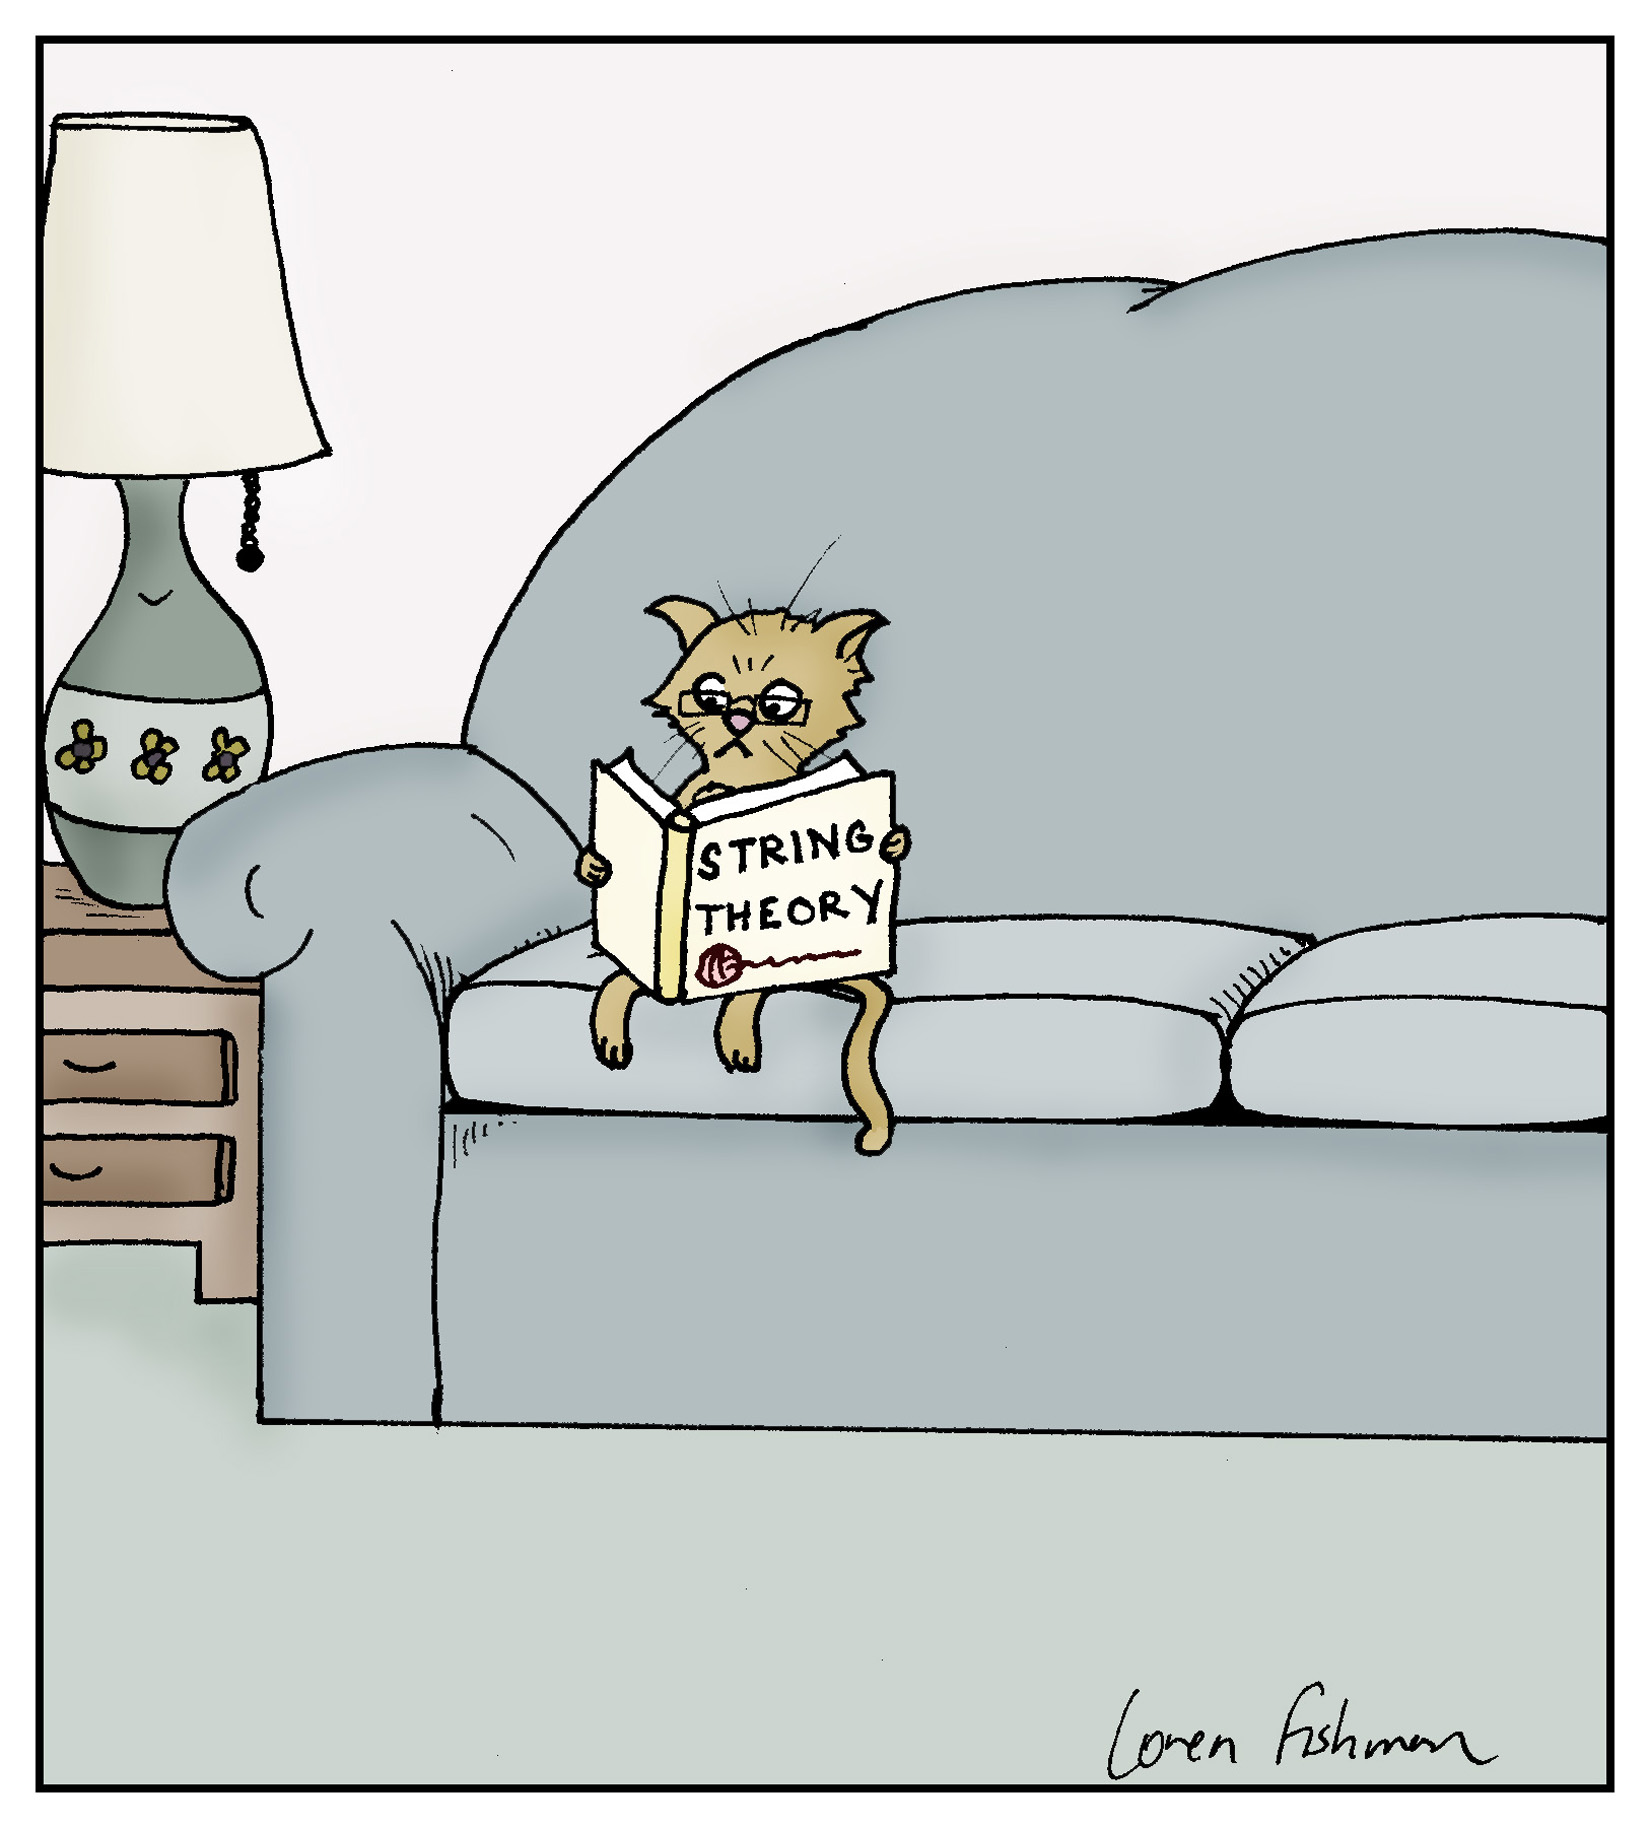
\includegraphics[width=0.43\textwidth]{string_cat.jpeg}
% \caption{
% What happened to Schrodinger's cat?
% }
% \label{fig:strings}
% \end{figure}

%==========================================================================
\section{Results}
\label{sec:results}
Here's what I found after I done'd it.

And Maxwell said:
\begin{gather}
    dF = 0, \\
    d_{\star}F = \mu_0 \, J.
\label{eq:doppler_mass}
\end{gather}
and then there was light.


%==========================================================================
\section{Conclusion}
\label{sec:conclusion}
Here's what you should learn now that I done'd it.


%==========================================================================
\begin{acknowledgments}
% Randos
We thank Bob Loblaw~\cite{BobLoblaw} for useful discussions.
% VV
V.V.~acknowledges support from NSF Grant No. PHY-2309301 and UMass Dartmouth’s
Marine and Undersea Technology (MUST) Research Program funded by the Office of
Naval Research (ONR) under Grant No. N00014-23-1–2141.
% LIGO
This material is based upon work supported by NSF's LIGO Laboratory which is a
major facility fully funded by the NSF.
% GWOSC
%This research made use of data, software and/or web tools obtained from the
%Gravitational Wave Open Science Center~\cite{GW_open_science_center}, a service
%of the LIGO Laboratory, the LIGO Scientific Collaboration and the Virgo
%Collaboration.
\end{acknowledgments}

%%%%%%%%%%%%%%%%%%%%%%%%%%%%%%%%%%%%%%%%%%%%%%%%%%%%%%%%%%%%%%%%%%%%%%%%%%%%%%%
\appendix
\section{Smooth Partitions of Unity}
\label{app:partitions_of_unity}
Partitions of unity are essential tools in the study of smooth manifolds, used to glue together objects defined locally to form global ones when the local objects do not agree on their common domain. Here, we provide a brief overview of smooth partitions of unity, which are used in the construction of the multi-domain surrogate model. 
%==========================================================================
\section*{References}
%%%%%%%%%%%%%%%%%%%%%%%%%%%%%%%%%%%%%%%%%%%%%%%%%%%%%%%%%%%%%%%%%%%%%%%%%%%%%%%
\bibliography{References}


\end{document}
